% ============================================
%       Presentation Compile Setting
% ============================================

\documentclass[8pt, aspectratio=169]{beamer} % for full presentation
% \documentclass[8pt, aspectratio=169, handout]{beamer} % without animation and notes
% \documentclass[8pt, aspectratio=169, handout, draft]{beamer} % for draft mode
% \documentclass[8pt, aspectratio=169, handout]{beamer} \setbeameroption{show only notes} % for notes only

% ============================================
%           MIC Lab template
% ============================================
\newcommand{\template}{../template}

% \input{\template/macros/macros_general.tex}
% \input{\template/macros/macros_math.tex}
% \input{\template/symbols/symbols_NN.tex}
% \input{\template/symbols/symbols_robot.tex}
% Add more macros/symbols as needed

\newcommand{\logoOne}{\template/figs/logo_KAIST_simple.png}
\newcommand{\logoTwo}{\template/figs/logo_MIC.png}
\newcommand{\logoTopRight}{\template/figs/logo_MIC_white.png}

% ============================================
%           Flux Theme
% ============================================

% Use roboto Font (recommended)
% \usepackage[sfdefault]{roboto}
\usepackage[utf8]{inputenc}
\usepackage[T1]{fontenc}

% Define where theme files are located. ('/styles')
\usepackage{styles/fluxmacros}
\usefolder{styles}
% Use Flux theme v0.1 beta
% Available style: asphalt, blue, red, green, gray, dding (custom)
\usetheme[style=dding]{flux}

% ============================================
%         Additional Packages
% ============================================

\usepackage{booktabs}
\usepackage{colortbl}
\usepackage{ragged2e}
\usepackage{schemabloc}
\usepackage{multirow}
\usepackage{multicol}
\usepackage{kotex}
\usepackage{media9}

% ============================================
%         Colors and Macros
% ============================================

% https://latexcolor.com % color list
\definecolor{airforceblue}{rgb}{0.36, 0.54, 0.66}
\definecolor{awesome}{rgb}{1.0, 0.13, 0.32}
\newcommand{\ctxt}[2]{{\color{#1}{#2}\color{black}}}
\newcommand{\cred}[1]{{\ctxt{awesome}{#1}}}
\newcommand{\cblue}[1]{{\ctxt{airforceblue}{#1}}}

% ============================================
%         Title Page
% ============================================
\title{
    Example of Presentation
} 
\subtitle{
    \textit{Where}\\
}
\author{
  \textbf{\cblue{Myeongseok Ryu}}\inst{1},  % Emphasize the presenter!
  % Jiyun Kim\inst{2},                      % Example of multiple institutes (see below)
  and 
  Kyunghwan Choi\inst{1}
}
\date{{\today} Change to presentation date!}
\institute{%
    \begin{minipage}[c]{\linewidth}
      \centering
      \inst{1}%
      Mobility Intelligence and Control Laboratory (MIC Lab) \\
      CCS Graduate School of Mobility \\
      Korea Advanced Institute of Science and Technology (KAIST)
      % Example of multiple institutes
      % \and 
      % \inst{2}%
      % AI Graduate School\\
      % Gwangju Institute of Science and Technology (GIST)
  \end{minipage}
}
\setbeamerfont{institute}{size=\normalsize}

\titlegraphic{\logoTopRight}

%~~~~~~~~~~~~~~~~~~~~~~~~~~~~~~~~~~~~~~~~~~~~~~~~~~~~~~~~~~~~~~~~~~~~~~~~~~~~~~
\AtBeginSection[]{%
  \frame<beamer>{ 
    \frametitle{Outline}   
    \tableofcontents[currentsection] 
  }
}

% Use the following code to show section and subsection titles at the beginning of each section and subsection
% \AtBeginSubsection[]{%
%   \begin{frame}
%   \vfill
%   \centering
%     \insertsectionhead
%     \\
%     \large\textbf{\insertsubsectionhead}
%   \vfill
%   \end{frame}
% }
%~~~~~~~~~~~~~~~~~~~~~~~~~~~~~~~~~~~~~~~~~~~~~~~~~~~~~~~~~~~~~~~~~~~~~~~~~~~~~~

\begin{document}

%~~~~~~~~~~~~~~~~~~~~~~~~~~~~~~~~~~~~~~~~~~~~~~~~~~~~~~~~~~~~~~~~~~~~~~~~~~~~~~
\titlepage 

\begin{frame}{Outline}
  \tableofcontents
\end{frame}
%~~~~~~~~~~~~~~~~~~~~~~~~~~~~~~~~~~~~~~~~~~~~~~~~~~~~~~~~~~~~~~~~~~~~~~~~~~~~~~

\section{Background and Contributions}

\subsection{Introduction to Neuro-Adaptive Control}

%~~~~~~~~~~~~~~~~~~~~~~~~~~~~~~~~~~~~~~~~~~~~~~~~~~~~~~~~~~~~~~~~~~~~~~~~~~~~~~
\begin{frame}{\insertsubsectionhead}{Example title}


  \vspace{0.5cm}

  \onslide<2-> % make animation like this
  {
    Insert figures like this:
    \begin{figure}
      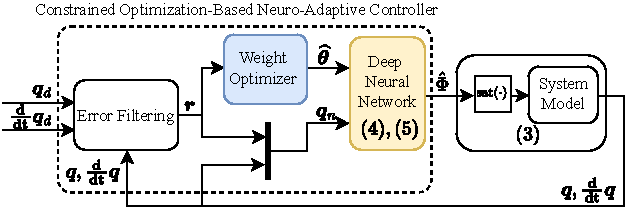
\includegraphics[width=0.45\textwidth]{figures/Controller.drawio.pdf}
      \caption{Example figure (CONAC).}
    \end{figure}
  }

  \onslide<3->
  {
    \begin{itemize}
      \item<3-> make animation of items like this
      \item<4-> by
      \item<5-> numbering!
    \end{itemize}
  }

\end{frame}

\note[enumerate]
{
  \item You can add notes like this.
  \item These notes will not be shown in the presentation.
}
%~~~~~~~~~~~~~~~~~~~~~~~~~~~~~~~~~~~~~~~~~~~~~~~~~~~~~~~~~~~~~~~~~~~~~~~~~~~~~~

%~~~~~~~~~~~~~~~~~~~~~~~~~~~~~~~~~~~~~~~~~~~~~~~~~~~~~~~~~~~~~~~~~~~~~~~~~~~~~~
\begin{frame}{You can remove subsection head}

  You can make multiple columns in a frame using the \texttt{columns} environment.

  \begin{columns}[T,onlytextwidth]

    \column{0.5\textwidth}

    \textbf{Left Column}

    \begin{itemize}
      \item Content1
      \item Content2
    \end{itemize}
    
    \column{0.5\textwidth}

    \textbf{Right Column}

    \begin{enumerate}
      \item Content3
      \item Content4
    \end{enumerate}

  \end{columns}
\end{frame}
%~~~~~~~~~~~~~~~~~~~~~~~~~~~~~~~~~~~~~~~~~~~~~~~~~~~~~~~~~~~~~~~~~~~~~~~~~~~~~~


%~~~~~~~~~~~~~~~~~~~~~~~~~~~~~~~~~~~~~~~~~~~~~~~~~~~~~~~~~~~~~~~~~~~~~~~~~~~~~~
\begin{frame}{\insertsubsectionhead}{Demonstration Video}

  Insert video like this:

  \centering
  \includemedia[
      width=0.64\linewidth,
      height=0.36\linewidth,
      activate=onclick,
      addresource=assets/animation.mp4,
      flashvars={
        source=assets/animation.mp4
        &autoPlay=true
        &loop=true
      }
    ]{}{VPlayer.swf}

\end{frame}
%~~~~~~~~~~~~~~~~~~~~~~~~~~~~~~~~~~~~~~~~~~~~~~~~~~~~~~~~~~~~~~~~~~~~~~~~~~~~~~

\section{Conclusion}

\subsection{Conclusion and Future Work}

%~~~~~~~~~~~~~~~~~~~~~~~~~~~~~~~~~~~~~~~~~~~~~~~~~~~~~~~~~~~~~~~~~~~~~~~~~~~~~~
\begin{frame}{Conclusion}

  You can use blocks like this 
  % block, alertblock, exampleblock

  \begin{block}{Block Title}
    Hi
  \end{block}

  \begin{exampleblock}{title}
    This is an example block.
  \end{exampleblock}

\end{frame}
%~~~~~~~~~~~~~~~~~~~~~~~~~~~~~~~~~~~~~~~~~~~~~~~~~~~~~~~~~~~~~~~~~~~~~~~~~~~~~~

%~~~~~~~~~~~~~~~~~~~~~~~~~~~~~~~~~~~~~~~~~~~~~~~~~~~~~~~~~~~~~~~~~~~~~~~~~~~~~~
\section{}
\begin{frame}{}
    \centering \Large
    \emph{Thank you for your attention!}
\end{frame}
%~~~~~~~~~~~~~~~~~~~~~~~~~~~~~~~~~~~~~~~~~~~~~~~~~~~~~~~~~~~~~~~~~~~~~~~~~~~~~~

%~~~~~~~~~~~~~~~~~~~~~~~~~~~~~~~~~~~~~~~~~~~~~~~~~~~~~~~~~~~~~~~~~~~~~~~~~~~~~~
\begin{frame}[allowframebreaks]{References}

  \bibliography{localRefs}
  \bibliographystyle{IEEEtran}

\end{frame}
%~~~~~~~~~~~~~~~~~~~~~~~~~~~~~~~~~~~~~~~~~~~~~~~~~~~~~~~~~~~~~~~~~~~~~~~~~~~~~~

%~~~~~~~~~~~~~~~~~~~~~~~~~~~~~~~~~~~~~~~~~~~~~~~~~~~~~~~~~~~~~~~~~~~~~~~~~~~~~~
\begin{frame}{Appendix}
  
  \textbf{If you need!} or remove this frame.

\end{frame}
%~~~~~~~~~~~~~~~~~~~~~~~~~~~~~~~~~~~~~~~~~~~~~~~~~~~~~~~~~~~~~~~~~~~~~~~~~~~~~~

\end{document}